\clearpage

\section{Детальный обзор LLVM}

LLVM (первоначально аббревиатура расшифровывалась как Low Level Virtual Machine) начался как
исследовательский проект Университета штата Иллинойс. Целью проекта было разработать промежуточное
представление (intermediate representation, IR), основанное на SSA (single static assignment) 
форме, способное описывать конструкции высокоуровневых языков программирования, а так же
универсальный набор оптимизаций над этим представлением. Неполный список проектов, входящих
в состав LLVM, включает в себя:

\begin{enumerate}
\item Ядро библиотеки, содержащее инструменты для работы с LLVM IR, а так же набор
оптимизаций и трансформаций над ним.
\item Clang -- фронтенд для C, C++ и Objective-C.
\item LLDB -- отладчик для C, C++ и Objective-C программ.
\item libc++ -- имплементация стандартной библиотеки C++.
\item OpenMP -- библиотеки времени исполнения для поддержки стандарта OpenMP.
\item LLD -- линковщик.
\item MLIR -- Multi-Level Intermediate Representation, набор библиотек для
создания собственных высокоуровневых промежуточных представлений и трансформаций
над ними. 
\end{enumerate}

\subsection{SSA форма}
% https://ru.wikipedia.org/wiki/SSA

\subsection{Just-in-Time компиляция}
% https://ru.wikipedia.org/wiki/JIT-%D0%BA%D0%BE%D0%BC%D0%BF%D0%B8%D0%BB%D1%8F%D1%86%D0%B8%D1%8F
\subsubsection{ORC JIT}
% https://llvm.org/docs/ORCv2.html

\subsection{Оптимизации во время компоновки}
% https://ru.wikipedia.org/wiki/%D0%9A%D0%BE%D0%BC%D0%BF%D0%BE%D0%BD%D0%BE%D0%B2%D1%89%D0%B8%D0%BA
\subsubsection{ThinLTO}
% https://clang.llvm.org/docs/ThinLTO.html
% http://blog.llvm.org/2016/06/thinlto-scalable-and-incremental-lto.html

\subsection{Clang}
% https://www.youtube.com/watch?v=5kkMpJpIGYU
% http://llvm.org/devmtg/2019-10/talk-abstracts.html#tut8
\subsubsection{Драйвер}
\subsubsection{Абстрактное синтаксическое дерево}
\subsubsection{Генерация кода}

\subsection{MLIR}
% https://mlir.llvm.org/
% http://llvm.org/devmtg/2019-04/talks.html#Keynote_1
\subsubsection{Диалекты}
% https://www.youtube.com/watch?v=ff3ngdvUang&feature=youtu.be
\begin{figure}[h]
    \centering
    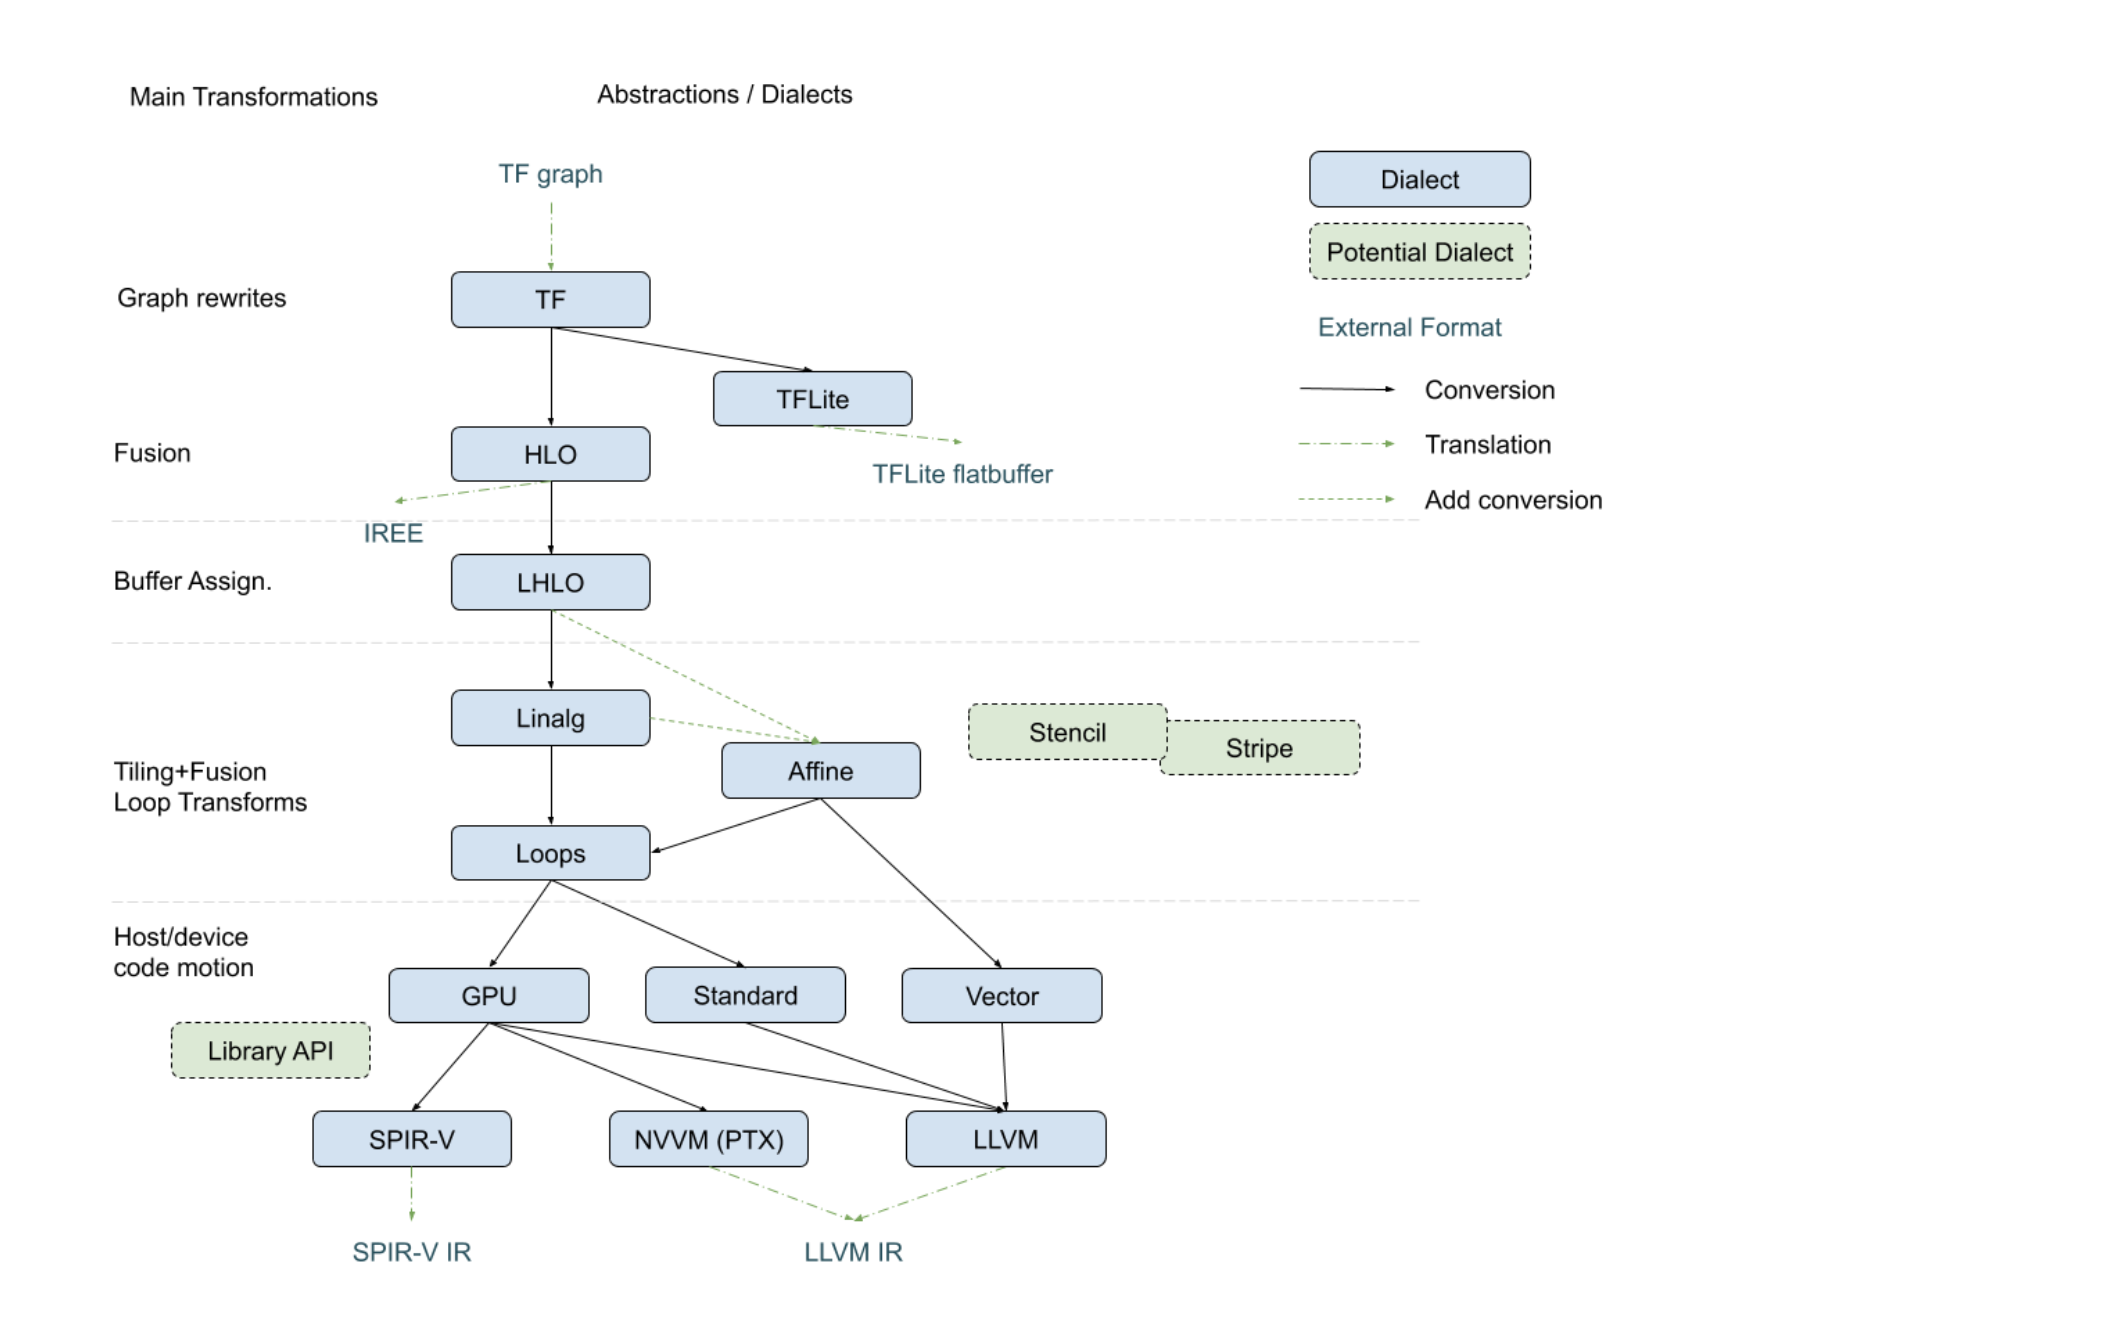
\includegraphics[width=\textwidth]{mlir_vector_dialect.png}
    \caption{Пример взаимодействия диалектов. Источник 
   % https://docs.google.com/presentation/d/1P-j1GrH6Q5gLBjao0afQ-GfvcAeF-QU4GXXeSy0eJ9I/edit#slide=id.p
    }
    \label{fig:mlir_vector_dialect}
\end{figure}
\subsubsection{Упрощенное полиэдральное представление}
% https://mlir.llvm.org/docs/Dialects/Affine/
